\section{Results and Discussion}
\label{sec:perovskites-results}

\subsection{Calculational Parameters}
The GPAW~\cite{gpaw-review-2010} DFT implementation was used with the same parameters as used in~\cite{double-defect-2011}.
Except that a tighter convergence criteria ($10^{-6} \unit{eV}$) for the electronic structure was used in order to reduce numerical noise.
The calculational supercell consisted of 2x2x2 formula units of \ce{SrTiO3} with a lattice constant of $3.931\unit{\mAA}$.

\subsubsection{Dimer Parameters}
The separation of the dimer images was set at $\Dsep = 0.001\unit{\mAA}$ and only one rotation per iteration was allowed, none if the rotational force was below $0.1\unit{eV/\mAA}$.
When determining the initial minimum modes and displacement away from minima, the defect hydrogen atoms were displaced using a Gaussian distribution with a standard deviation of $0.01 \unit{\mAA}$ in each direction.

\subsection{Searching for Diffusional Mechanisms}
The results of \cite{double-defect-2011} showed that the hydrogen atoms would move in individual steps while staying close to each other.
Two such mechanisms were discussed and both consisted of multiple iterations of two types of events.
Either the transitioning hydrogen atom would "jump" from one oxygen atom to the next near a titanium atom (as seen for atom A in \fref{fig:jump-combined}) or it would "rotate" past a strontium atom while remaining near the same oxygen atom (as seen for atom B in \fref{fig:jump-combined}).
Both hydrogen atoms would perform these steps --- often in alternating order --- while remaining in close proximity of each other, to diffuse through the system.

Dimer \sap{1} searches were conducted, starting from the various minima suggested in \cite{double-defect-2011}.
Essentially, confirming the previous results, the low energy \sap{1}s were all events of the types described above.
Only a handful of truly concerted events, where both hydrogen atoms would transition simultaneously, were detected but they were all higher in energy.
%A few low energy \sap{1}s were found for slight lattice rearrangement

Some \sap{1}s were found at a slightly longer range, e.g. where the hydrogen atoms would be separated by a strontium atom.
In the calculational cell used this is effectively half of its length, bringing into question any discussion on the energies as periodic effects could both over- and underestimate the stabilisation by the neighbouring hydrogen atom.
Further investigation of these might prove interesting but a larger calculational cell is required.

\subsection{DFT Ridge Calculations}
The same parameters were used for the dimer part of the ridge calculations as were used for the dimer searches above.

A few ridge calculations were started with some of the \sap{1}s found above as endpoints.
The general results can be split into three categories.
\bit
\item Successful ridge calculations, converged from a linear interpolation to a ridge in under 300 iterations.
\item Unsuccessful calculations where the path would spent most of its time as an inverted barrier near the minimum energy path.
\item Calculations where a soft eigenmode was followed resulting in a non-converging calculation where the lattice would distort heavily.
\eit

\subsubsection{Successful DFT Ridge Calculations}
\begin{figure}[h]
\begin{center}
  \subfigure[The configuration of the A-jump \sap{1}. One titanium atom is semi-transparent to allow viewing of hydrogen B]{
    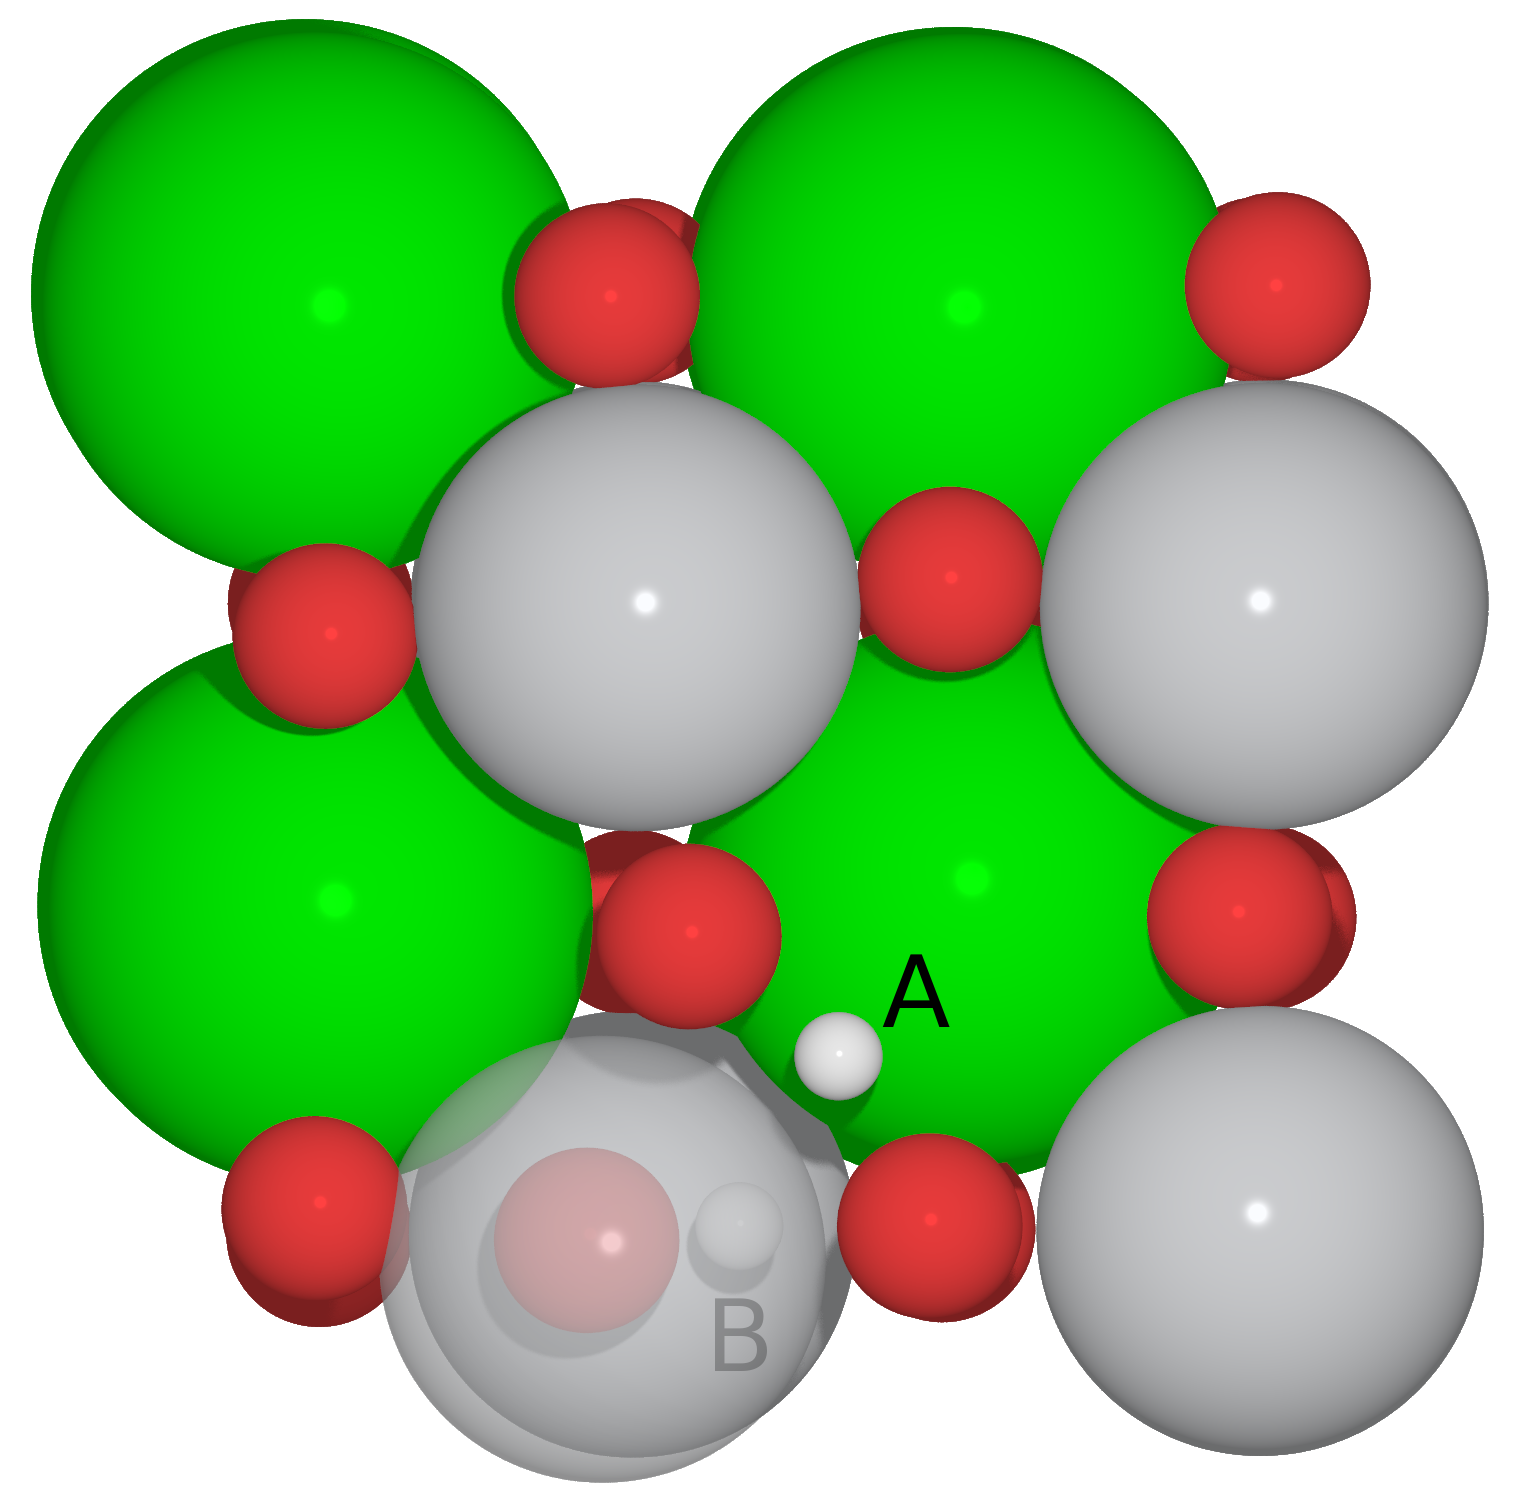
\includegraphics[width=0.45\linewidth]{semi-combined}
    \label{fig:semi-combined}
    }
  \subfigure[Energy profile of the ridge]{
    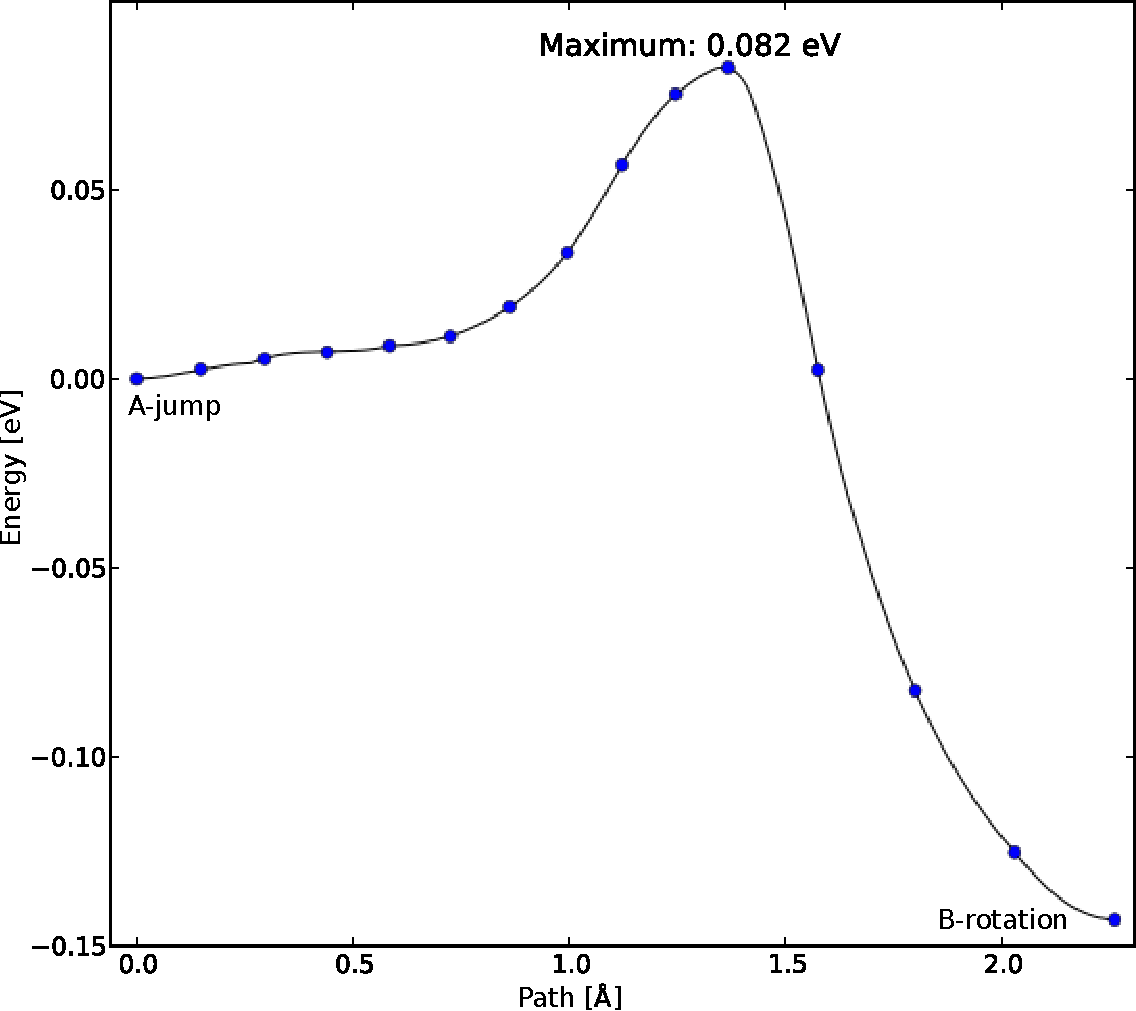
\includegraphics[width=0.45\linewidth]{semi-ridge}
    \label{fig:semi-ridge}
    }
    \parbox{0.85\linewidth}{
      \caption{A successful DFT ridge calculation between a jump \sap{1} for hydrogen atom A and rotation of hydrogen atom B.
The hydrogen atoms are white, the titanium atoms are grey, the strontium atoms are green and the oxygen atoms are red.
      }
      \label{fig:semi-results}
    }
\end{center}
\end{figure}
\begin{figure}[h]
\begin{center}
  \subfigure[The configuration of the A-jump/B-rotate \sap{2}. One strontium atom removed is semi-transparent to allow viewing of the hydrogen atoms]{
    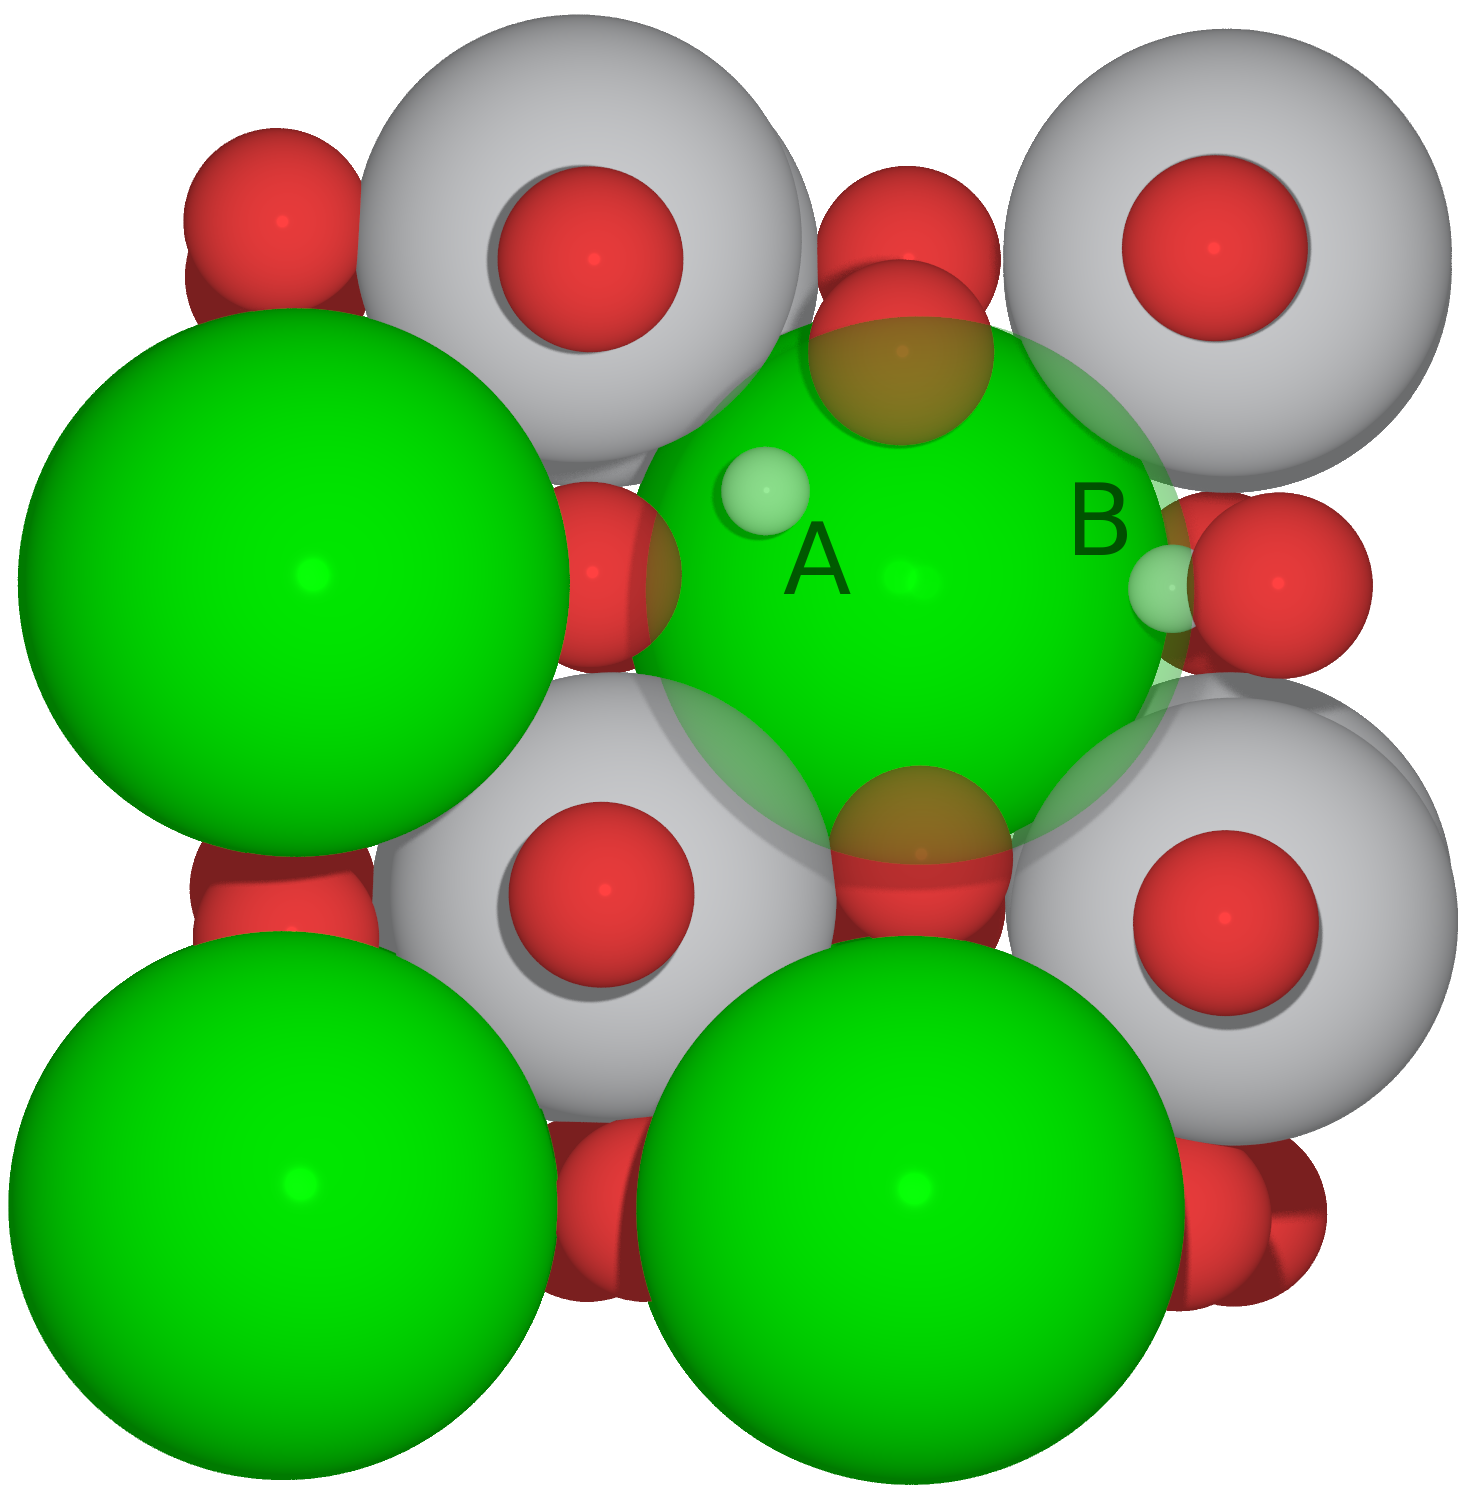
\includegraphics[width=0.45\linewidth]{jump-combined}
    \label{fig:jump-combined}
    }
  \subfigure[Energy profile of the ridge]{
    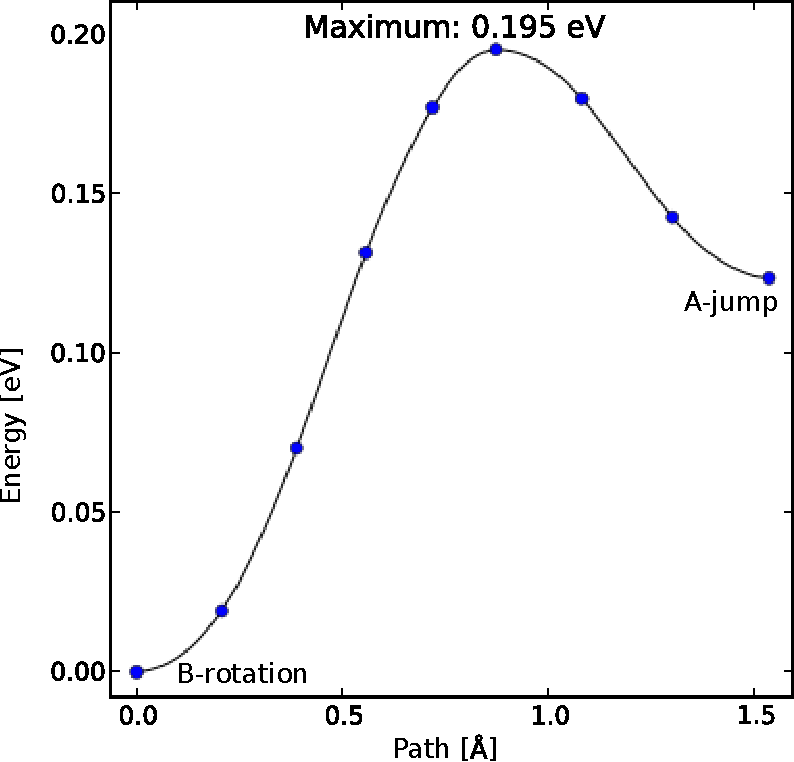
\includegraphics[width=0.45\linewidth]{jump-ridge}
    \label{fig:jump-ridge}
    }
    \parbox{0.85\linewidth}{
      \caption{A successful DFT ridge calculation between a jump \sap{1} for hydrogen atom A and rotation of hydrogen atom B.
The hydrogen atoms are white, the titanium atoms are grey, the strontium atoms are green and the oxygen atoms are red.
      }
      \label{fig:jump-results}
    }
\end{center}
\end{figure}
The most interesting of the successful ridge calculations was one where the ridge near a jump-type \sap{1}s (\fref{fig:semi-combined}) consisted of a rather flat energy profile (\fref{fig:semi-ridge}) with lattice rearrangement before a sharp rise to reach a $0.08\unit{eV}$ \sap{2} on its way to a rotation-type \sap{1} for the other hydrogen atom.
A second successful calculation of the ridge near a different jump-type \sap{1} revealed one other low energy \sap{2} of $0.08\unit{eV}$. (\fref{fig:jump-results})
Both the \sap{2}s are outside the $5\kB T$ limit but finding multiple low energy \sap{2}s and a flat energy profile are clear warning signs, that the HTST rate could be improved.

From an informal visual inspection of the successful ridge calculations, the initial paths never lay close to a minimum.
However, it was not possible to make the opposite claim for the failed calculations.

\subsubsection{Basin Trapped Paths}
Those calculations that did not reach the ridge, generally lay near the minimum energy path and were not able to rise out of the basin.
The eigenvalue estimate would remain negative for most of the images.

It is unlikely that this minima-trapping behaviour is an artefact of the method itself as such things did not happen in the previous test cases.
More, likely is that the DFT parameters must be further considered.
A significant eggbox effect~\cite{gpaw-2005} was seen when relaxing the structures.
Even though the dimer searches were not affected in an obvious manner, this could affect the ridge calcualtions, due to the correlated nature of the images.
%It is not unthinkable that this results in an artificial ridge which may be found.
Furthermore, a rather large gridspacing ($0.2 \unit{\mAA}$ was used, further reducing the accuracy of the forces.
Nevertheless, neither of these can be identified as the cause of the failed calculations without further research.

\subsubsection{Soft Minimum modes}
Latching on to a soft minimum mode is a concern that is always possible with dimer-type algorithms.
However, this was not a significant problem in the previous tests.
In this particular case, the climbing image had been turned on very early in order to avoid the basin trapping problem.
After the climbing image is turned on with a soft minimum mode, the calculation is unlikely to yield an interesting result.
This problem raises questions about the initial minimum modes.
If a random initial minimum mode is used (as was the case in this calculation), is it likely that neighbouring minimum modes will not be similar (i.e. not find the same ridge).
It is of course possible to initialise the minimum modes in a linear fashion, using the unstable modes of the end points or implement some constraint to avoid neighbouring minimum modes from from being dissimilar.
In any case, this warrants further consideration.

\subsection{Summary}
Neither the dimer searches nor the ridge calculations found interesting pathways beyond those suggested by~\cite{double-defect-2011} and thus it can be concluded that their picture of the diffusion is accurate.
Since the low energy \sap{2}s were found near different \sap{1} for a similar event, it is reasonable to assume that similar \sap{2}s exist near the jump event of an isolated defect.
Thus, there is no reason to conclude that the ratio of mobilities is different from the reported one without further ridge calculations in both systems.
A coupled defect has slightly higher mobility than an isolated one.

Out of 7 ridge calculations, only 3 were successful, while 1 followed a soft minimum mode and 3 were trapped in basins.
Despite the failed calculations, there were successful ones which converged to the ridge and the \sap{2}s of a highly complex DFT system.
Further testing is, of course, needed to fully understand the flawed calculations.
Nevertheless, the interesting results remain.
Warning flags must be raised when considering the harmonicity of the jump-type transitions.
